% !TeX spellcheck = en_US


\chapter{Hardware Design}


\section{Magnetically transduced whisker sensor}
The structure of a single whisker sensor is shown in \cref{fig:whisker_composite}.

\begin{figure}[ht]
    \centering
    \begin{subfigure}{0.31\textwidth}
        \centering
        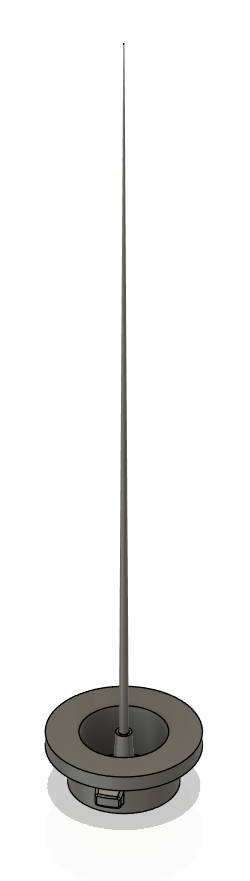
\includegraphics[height=0.2\textheight]{figures/whisker}
        \caption{Whisker mounted on the suspension} \label{fig:whisker}
    \end{subfigure}
    \hspace*{\fill}
    \begin{subfigure}{0.31\textwidth}
        \centering
        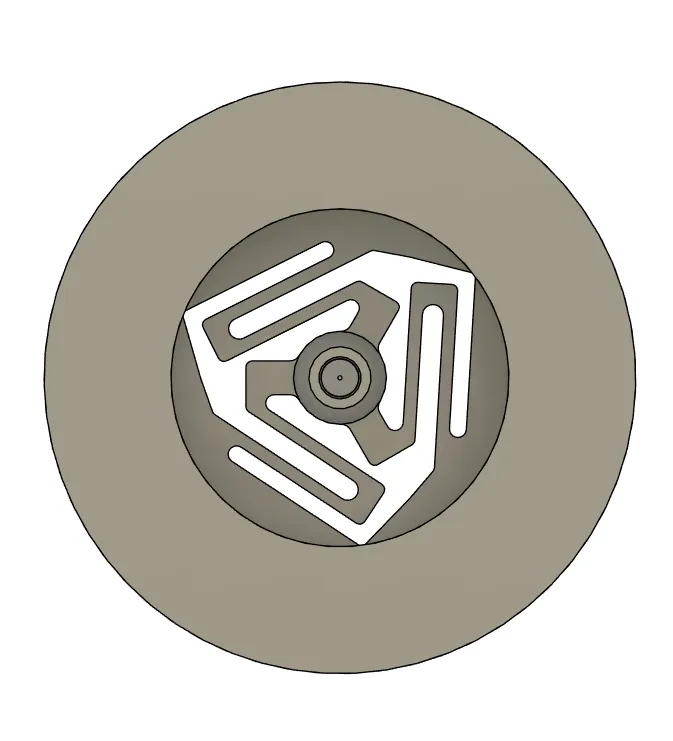
\includegraphics[width=\linewidth]{figures/suspension}
        \caption{Suspension Design} \label{fig:suspension}
    \end{subfigure}
    \hspace*{\fill}
    \begin{subfigure}{0.31\textwidth}
        \centering
        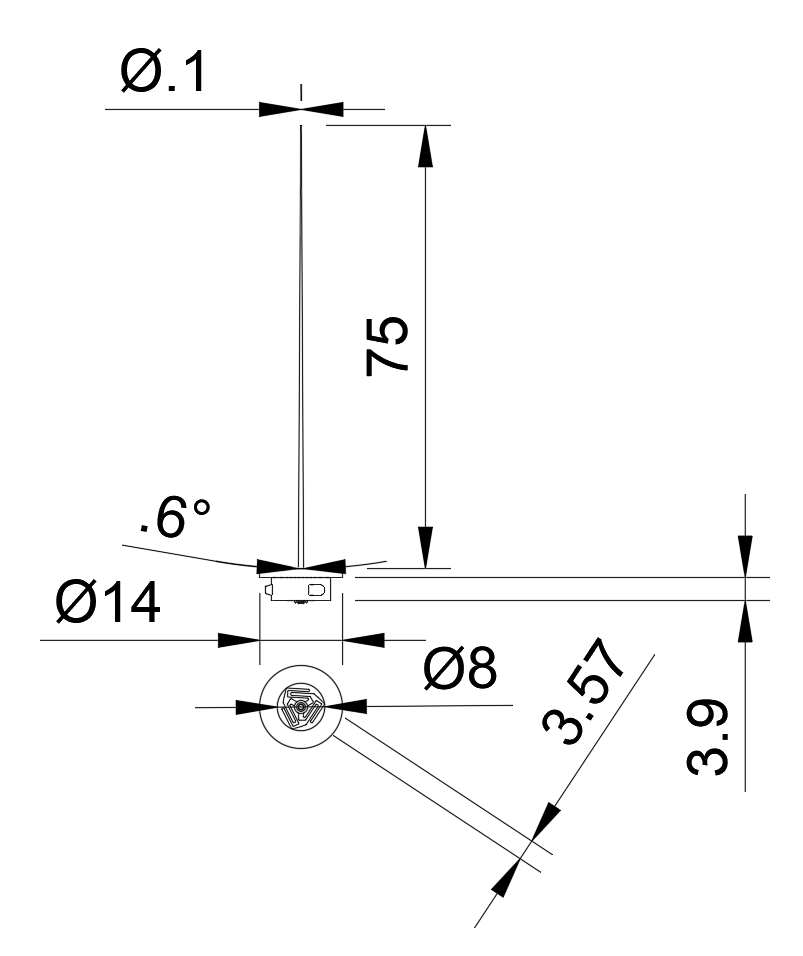
\includegraphics[width=\linewidth]{figures/whisker-dims}
        \caption{Structure dimensions} \label{fig:whisker-dims}
    \end{subfigure}
    \caption{Single whisker sensor.}
    \label{fig:whisker_composite}
\end{figure}

The whisker consists of:
\begin{itemize}
    \item A flexible whisker shaft made of a nitinol wire (0.25 mm diameter, 75 mm length).
    \item A suspension system fabricated via 3D printing using PLA plastic as filament.
    \item A magnetic sensor Adafruit MLX90393, configured for measuring magnetic flux changes with resolution of 0.15 $\micro T/LSB$
\end{itemize}
The whisker shaft is first inserted and glued to the suspension system.
A neodymium permanent magnet, axially magnetized with its field direction aligned with the wire, is placed underneath the suspension below the whisker shaft.
As the whisker deflects, the magnet rotates in place, causing a change in the magnetic field.


\section{Whisker Platform}

A whisker platform was developed to allow multi-whisker exploration and reconstruction.
It consists of a triangularly-shaped body with 30\degree nose, two side clamps, which allow for 3 whiskers to be attached on each side, and a mount for the Franka Panda robotic arm with a gripper.
The platform, show on the Figure~\cref{fig:platform}, has a size of 90 mm x 60 mm x 35 mm and is 3D printed using PLA plastic filament.
Figure~\ref{fig:whisker_platform} showcases the 3D-printed version of the same platform.
The platform is designed to resemble the shape of the rat, even if just roughly.

The MLX90393 sensors are being held in place by the side clamps.
The cuts in the clamps allow for 4-ping JST connectors to be used on both sides of the sensors.
All the components are hold together by M2 and M3 screws.

The clamps and suspension bases are designed in such a way, that the whiskers can be plugged into the holes in the clamps and locked by slight rotation.
The whiskers can be easily replaced the same way.
No external power supply apart from the JST connector is needed.

The whisker mounts are positioned at an angle of 15\degree to the mirror plane of the platform.
This allows for a larger contact search space, as the whiskers point slightly forward.
The downside of such placement is that, especially in tunneling scenarios, the whiskers can get face the object head-on and deflect in the opposite direction.
Too severe deflection can cause the whisker to break or deform permanently, therefore safeguards in the control system are needed to prevent such behavior.
This is outside the scope of this thesis, and in the simulation because of the same reason the whiskers are pointed slightly backwards.

\begin{figure}[ht]
    \centering
    \begin{subfigure}[b]{0.45\textwidth}
        \centering
        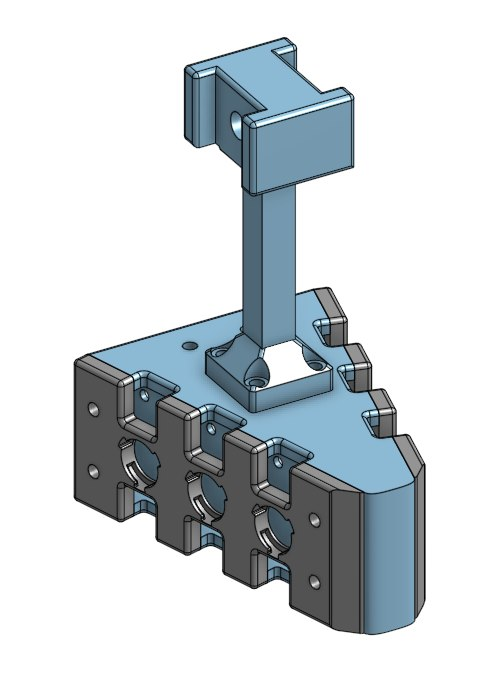
\includegraphics[height=0.3\textheight]{figures/platform-cad}
        \caption{Platform CAD model.}
    \end{subfigure}
    \hfill
    \begin{subfigure}[b]{0.45\textwidth}
        \centering
        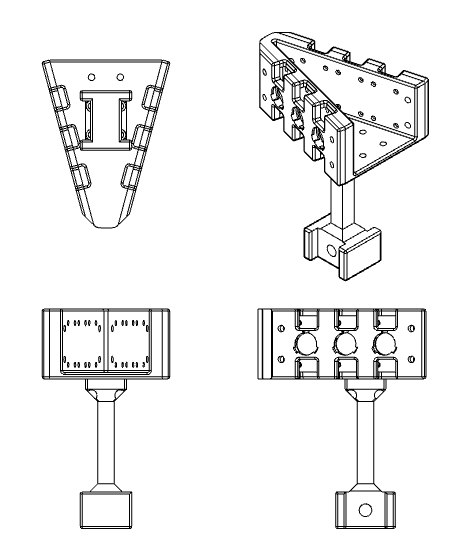
\includegraphics[height=0.3\textheight]{figures/platform-sketch}
        \caption{Platform sketch from below.}
    \end{subfigure}
    \caption{Whisker platform CAD model and sketch.}
    \label{fig:platform}
\end{figure}

\begin{figure}[htb]
    \centering
    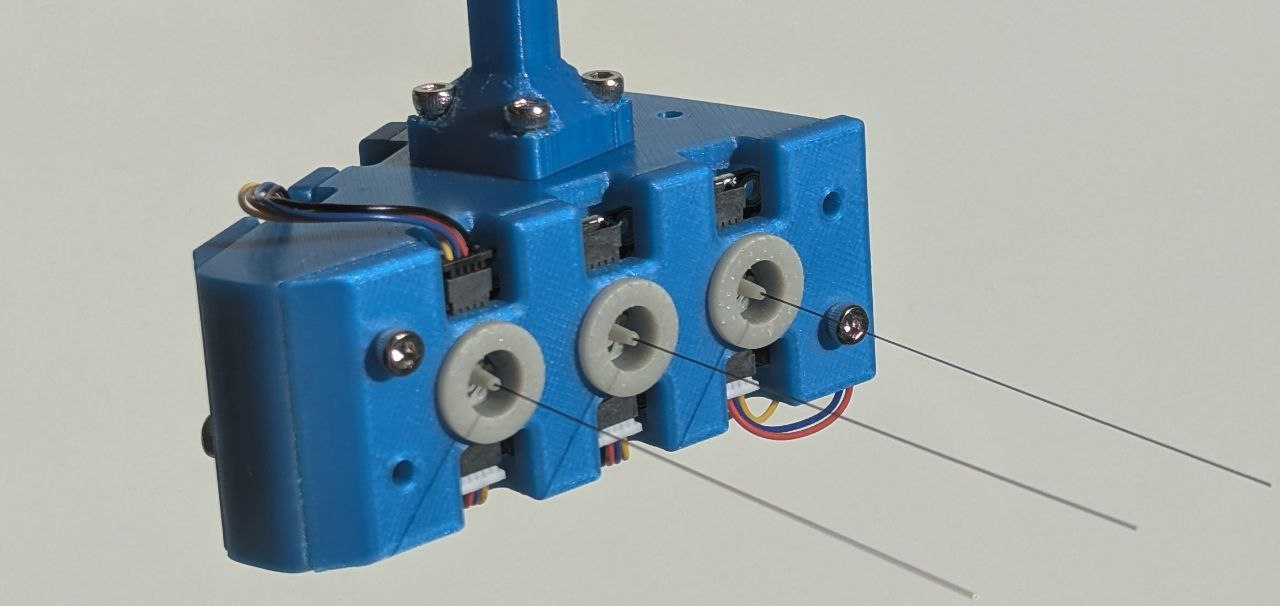
\includegraphics[width=0.6\textheight]{figures/platform}
    \caption{Whisker platform with three whiskers and robotic arm mount attached.}
    \label{fig:whisker_platform}
\end{figure}


\section{Data Acquisition}

Adafruit MLX90393 devboard, shown on the Figure~\cref{fig:sensor} hosting a Hall sensor is located 2--3mm underneath the magnet glued to the suspension.
The sensor uses a 16-bit ADC with proportional output of the magnetic flux density sensed along the XYZ axes.
It is configured for measurement with a resolution of \(0.15 \mu T/LSB\).
In fact, only Z component is used, as it unambiguously captures the rotating caused by planar whisker deflections.
The sensor uses I2C communication protocol, acting as a slave.
If multiple sensors are used, they are connected in a daisy chain.

Two MLX90393 sensor drivers have been implemented: one in C++ for the ESP32 microcontroller and another in Python for the Raspberry Pi 5.
They are based on the official MLX90393 Triaxis® Magnetic Node specification~\cite{MLX90393}.
Continuous burst mode is used to read the sensor data, as points at equal time intervals are needed for the control loop.
This allows to read our the data at a rate of 300Hz.
This rate allows for filtering of the deflection signal at fast-paced movements.
The control loops itself runs at around 30Hz, as this is the limit at which the actuator can be controlled.

\begin{figure}[ht]
    \centering
    \begin{subfigure}[b]{0.45\textwidth}
        \centering
        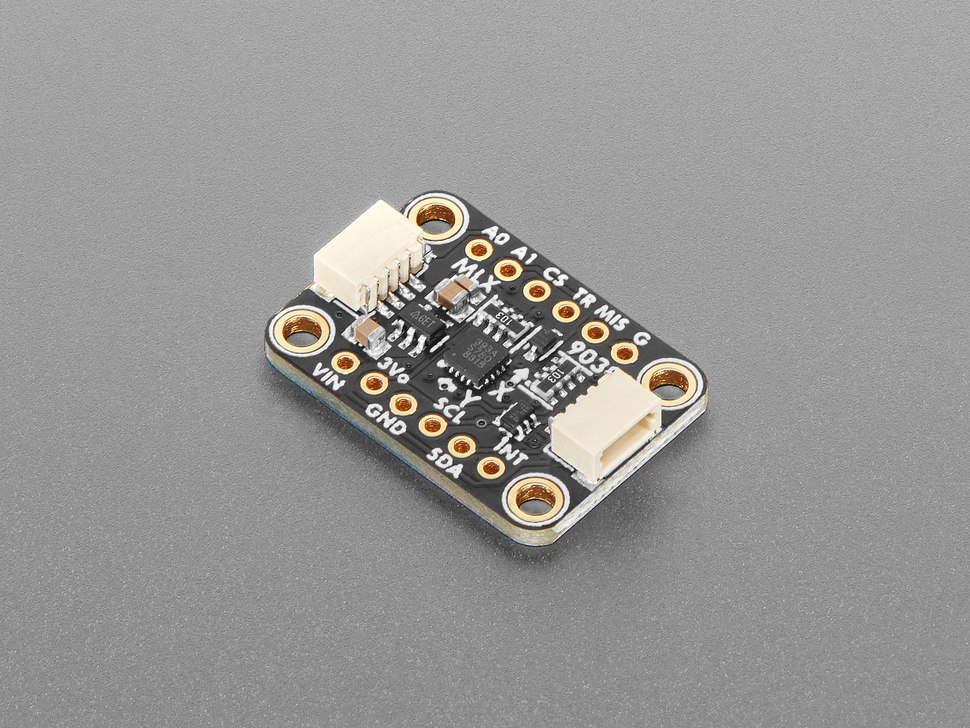
\includegraphics[width=\linewidth]{figures/mlx90393}
        \caption{Adafruit MLX90393 devboard, 25.4mm x 17.8mm x 1.6mm, from~\cite{MLX90393}}
    \end{subfigure}
    \hfill
    \begin{subfigure}[b]{0.45\textwidth}
        \centering
        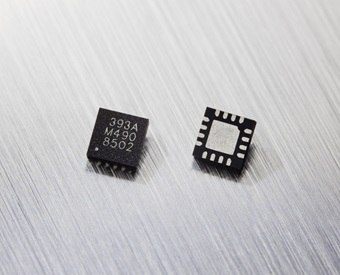
\includegraphics[width=\linewidth]{figures/mlx90393-chip}
        \caption{Melexis MLX90393 chip, 3.1mm x 2.9mm x 1mm, from~\cite{MLX90393}}
    \end{subfigure}
    \label{fig:sensor}
\end{figure}

To convert the magnetic field strength into whisker deflection a calibrated deflection model is used.
It is created by sampling the sensor readouts at different deflection angles and fitting a 5th degree polynomial to the data.
Although this approach is not very precise at the whole range of deflections, it covers the normal operation range of deflection, which is around -5e-4--5e-4 rad, is sufficient for the purpose of this thesis.
The deflection model is shown in Figure~\ref{fig:deflection_profile}.
It mirrors the deflection offset from the neutral position and clips the result based on the whisker's half-circle limit to stabilize points outside the range of operation.

\begin{figure}[htb]
    \centering
    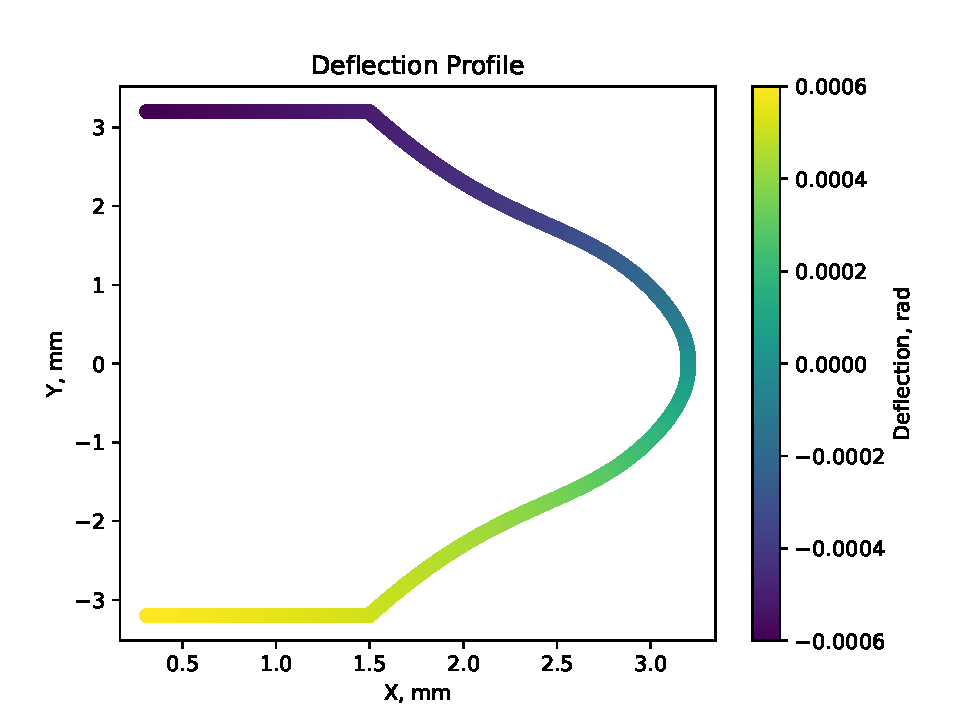
\includegraphics[width=0.8\textwidth]{figures/deflection_profile}
    \caption{Deflection Profile Model.}
    \label{fig:deflection_profile}
\end{figure}
